% Latex template: mahmoud.s.fahmy@students.kasralainy.edu.eg
% For more details: https://www.sharelatex.com/learn/Beamer

\documentclass[aspectratio=1610]{beamer}					% Document class

\setbeamertemplate{footline}[text line]{%
  \parbox{\linewidth}{\vspace*{-8pt}Deep methods for interpretable analysis of gene interactions\hfill\insertshortauthor\hfill\insertpagenumber}}
\setbeamertemplate{navigation symbols}{}

\usepackage[english]{babel}				% Set language
\usepackage[utf8x]{inputenc}			% Set encoding

\mode<presentation>						% Set options
{
  \usetheme{default}					% Set theme
  \usecolortheme{default} 				% Set colors
  \usefonttheme{default}  				% Set font theme
  \setbeamertemplate{caption}[numbered]	% Set caption to be numbered
}

% Uncomment this to have the outline at the beginning of each section highlighted.
%\AtBeginSection[]
%{
%  \begin{frame}{Outline}
%    \tableofcontents[currentsection]
%  \end{frame}
%}

\usepackage{graphicx}					% For including figures
\usepackage{booktabs}					% For table rules
\usepackage{hyperref}					% For cross-referencing
\usepackage[absolute,overlay]{textpos}

\title{Deep methods for interpretable analysis of gene interactions}	% Presentation title
\author{Clayton W. Seitz}								% Presentation author
\date{\today}									% Today's date	

\begin{document}

% Title page
% This page includes the informations defined earlier including title, author/s, affiliation/s and the date
\begin{frame}
  \titlepage
\end{frame}

% Outline
% This page includes the outline (Table of content) of the presentation. All sections and subsections will appear in the outline by default.
\begin{frame}{Outline}
  \tableofcontents
\end{frame}

% The following is the most frequently used slide types in beamer
% The slide structure is as follows:
%
%\begin{frame}{<slide-title>}
%	<content>
%\end{frame}


\begin{frame}{The logic of generative modeling}

Say we have a set of variables $\mathbf{x} = (x_{1},x_{2},...,x_{n})$ which might have some statistical dependence\\
\vspace{0.1in}
The variable $\mathbf{x}$ might be an amino acid sequence, gene expression data, microscopy image, etc.\\
\vspace{0.1in}
\begin{itemize}
\item Often we are handed a batch of empirical samples $\{\mathbf{x}_{i}\}_{i=1}^{N}$
\item We want to know the generating distribution $p(\mathbf{x})$
\end{itemize}

In supervised \textcolor{red}{generative learning}, we try to explicity learn the joint distribution $p(\mathbf{x}) = \prod_{i=1}^{N-1}p(x_{i}|x_{i+1:N})p(x_{N})$, which is generally more difficult than discriminative learning. 

\end{frame}

\begin{frame}{Generative modeling with feedback}
\begin{figure}
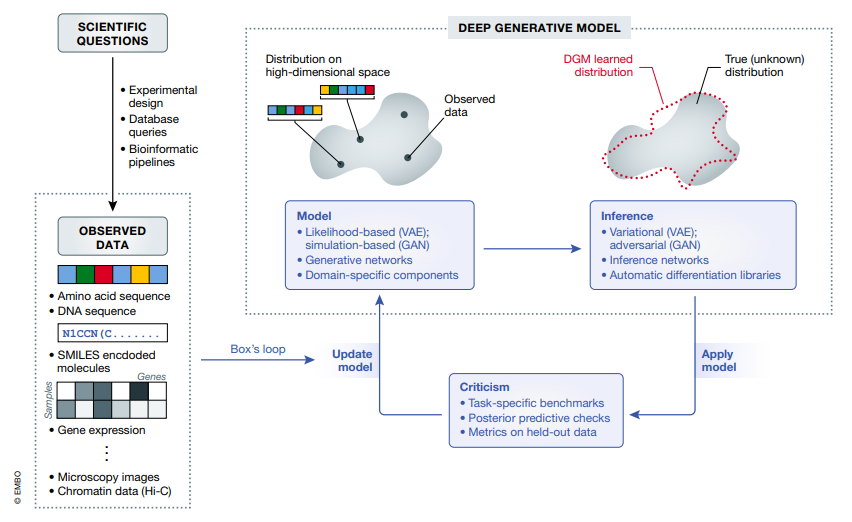
\includegraphics[height=65mm, width=105mm]{dbm}
\end{figure}
\end{frame}



\begin{frame}{Perks of generative modeling}

\begin{itemize}
\item Fitting complete multivariate distributions $p(\mathbf{x})$ goes beyond correlation-based or clustering approaches
\item Correlations cannot discover partial correlation in the context of other neighbors
\item Fitting $p(\mathbf{x})$ permits sampling based inference
\end{itemize}

\end{frame}


%\section{The variational autoencoder}
%\begin{frame}{Variational autoencoders (VAEs)}
%A variational solution to generative modeling
%
%\begin{center}
%\begin{figure}
%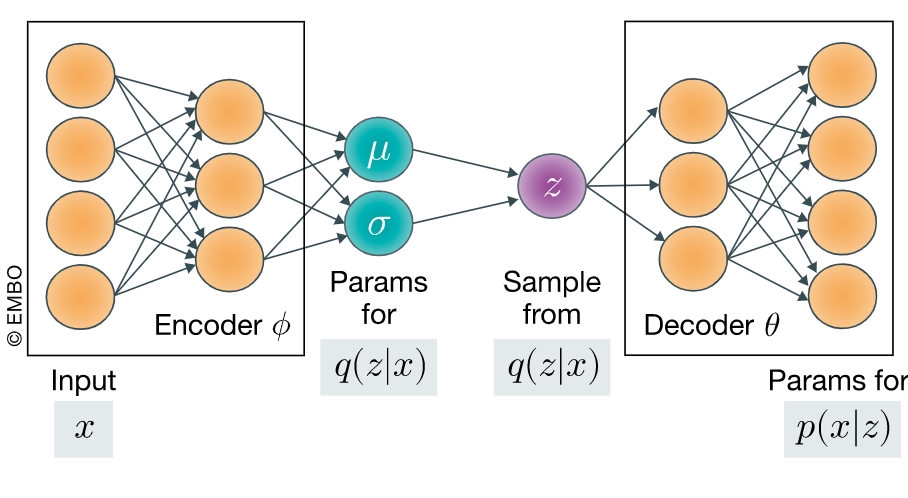
\includegraphics[width=0.9\textwidth]{vae}
%\caption{\textbf{Variational autoencoder architecture} Taken from Lopez 2020 in EMBO}
%\end{figure}
%\end{center}
%\end{frame}

\begin{frame}{Gene interactions are naturally represented as graphs}

\end{frame}

\section{Graph convolutional networks}

\begin{frame}{Quick review of convolutional neural networks}

Assume stationarity of image statistics and locality of pixel dependencies

\end{frame}

\begin{frame}{Defining Graph Convolution}
Can be viewed as a generalization of convolutional neural networks to graph structured data

\begin{textblock*}{5cm}(1cm,5cm)
\begin{equation*}
y = mx+b
\end{equation*}
\end{textblock*}

\begin{textblock*}{5cm}(7.5cm,0.5cm)
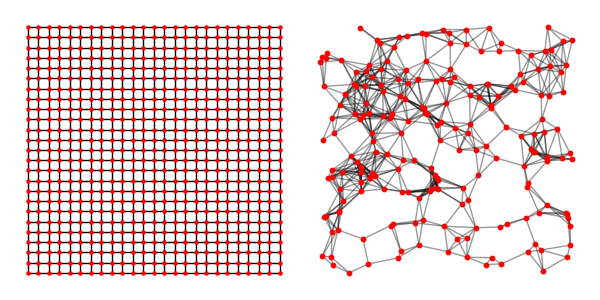
\includegraphics[width=7cm]{graphs.png}
\end{textblock*}

\end{frame}

\begin{frame}{Learning Bayesian network structure}

\end{frame}

\begin{frame}{Directed graph convolution on Bayesian networks}

\end{frame}

\section{References}

% Adding the option 'allowframebreaks' allows the contents of the slide to be expanded in more than one slide.
\begin{frame}[allowframebreaks]{References}
	\tiny\bibliography{references}
	\bibliographystyle{apalike}
\end{frame}

\end{document}